
% Author: PokMan Ho pok.ho19@imperial.ac.uk
% Script: LogisticTmp.tex
% Desc: `LaTex` report framework -- Logistic Growth
% Input: none
% Output: none
% Arguments: 0
% Date: Oct 2019

\documentclass[a4paper, 11pt]{article}
\usepackage[margin=1in]{geometry}
\usepackage{hyperref, setspace, lineno}

%% test insert graphs
\usepackage{graphicx}
\graphicspath{ {../results/} } %% <https://www.overleaf.com/learn/latex/Inserting_Images>

%% test insert variables
\newcommand{\ReportTitle}{Report on Model Selection between Logistic Growth curves based on chosen Bacterial Population Growth Experimental Data} %% <https://stackoverflow.com/questions/1211888/is-there-any-way-i-can-define-a-variable-in-latex>
\newcommand{\ReportAuthor}{PokMan HO}
\newcommand{\ReportAffil}{Department of Life Sciences, Faculty of Natural Sciences,\\Imperial College London}
\newcommand{\Disclaim}{\textbf{A Mini-project submitted in partial fulfilment of the requirements for the degree of Master of Research at Imperial College London\\\\Formatted in the journal style of the \textit{Nature} Journal\\Submitted for the MRes in Computational Methods of Ecology and Evolution}}

\title{\ReportTitle}
\author{\ReportAuthor (CID: 01786076)}
\date{}

%% citation
\usepackage[%
autocite    = superscript,
backend     = bibtex,
sortcites   = true,
style       = nature
]{biblatex}
\bibliography{../reference/LogRef.bib} %% <https://tex.stackexchange.com/questions/6805/bib-library-file-in-a-different-directory-how-to-use-mendeley-centralised-b>

%% set as required
\doublespacing
\linenumbers

\begin{document}
	\begin{center}
		\Huge\textbf{\ReportTitle}\\
		\LARGE\ReportAuthor\\
		\Large\ReportAffil
	\end{center}
	\begin{figure}[h]
		\centering
\includegraphics[width=\linewidth]{icl.jpg}
	\end{figure}
	\begin{flushright}
		\Large Approximate Word Count: %% insert approx word count
	\end{flushright}
	\clearpage
	
	\maketitle
	\section*{Abstract}
	
	
	\section*{Introduction}
	Multiple equations are published attempting to describe the logistic growth pattern of microbes.  Limited by the research scales, these equations may not always align perfectly with all microbial growth datasets.  This report is aimed at choosing one dataset from a published article and apply non-linear least square (NLLS) model selection method to compare their descriptive effectiveness on this chosen dataset.
	
	\section*{Methods}
	A subset of microbial growth data was selected based on ``the highest number of data points".  The candidate dataset was the replicate %1 %%%%%%% FIRST CUT AFTER THIS %%%%%%%
	 from Zwietering \textit{et al.}(1994)\autocite{zwietering1994modeling} \textit{%L.plantarum
	}on %MRS
	 substrate under %10
	 degrees Celsius.  The data was containing %151
	 records on population cell count (%N
).\\
	The data was recorded in ``population change" (response variable) against ``time of experiment (hr)" (explanatory variable).  The response variable was neither normally-distributed nor log-normal (Shapiro Test p-value: %0
	; Min
	, 1st Q
	, 2nd Q
	, 3rd Q
	, Max
	, all corrected to 2 d.p.).  Time (in hr) was also recorded not in a normal-distributed not log-normal way (Shapiro Test p-value: %0
	; Min
	, 1st Q
	, 2nd Q
	, 3rd Q
	, Max
	, all corrected to 2 d.p.).\\
	Expected population change calculated from Verhulst equation (classical logistic model)\autocite{mckendrick1912xlv}, modified Gompertz model\autocite{GIL200689}, Baranyi model\autocite{baranyi1993modeling} and Buchanan model\autocite{buchanan1993differentiation} were plotted against the real data on a semi-log graph of ``log Population Change" vs ``Time (hr)".  The mechanistic models were also evaluated by NLLS method\autocite{kelley1999iterative,strutz2010data}.  Pairwise comparisons of models with AIC\autocite{akaike1998information,burnhamdr} and BIC\autocite{schwarz1978estimating} selection methods were also carried out for identification of fittest model the the chosen dataset.
	\subsection*{Computing tools}
	R (ver 3.6.0)\autocite{Rcore} was used with following packages: ``ggplot2"\autocite{ggplot2} was used for visualisation; ``reshape2"\autocite{reshape2} was used for converting dataset from wide to long format; ``scales"\autocite{scales} was used for improve ``ggplot" graphs data presentation; and ``minpack.lm"\autocite{minpacklm} was used for computing non-linear least square statistics for model comparisons.
	
	\section*{Results}
	\begin{figure}[h]
		\centering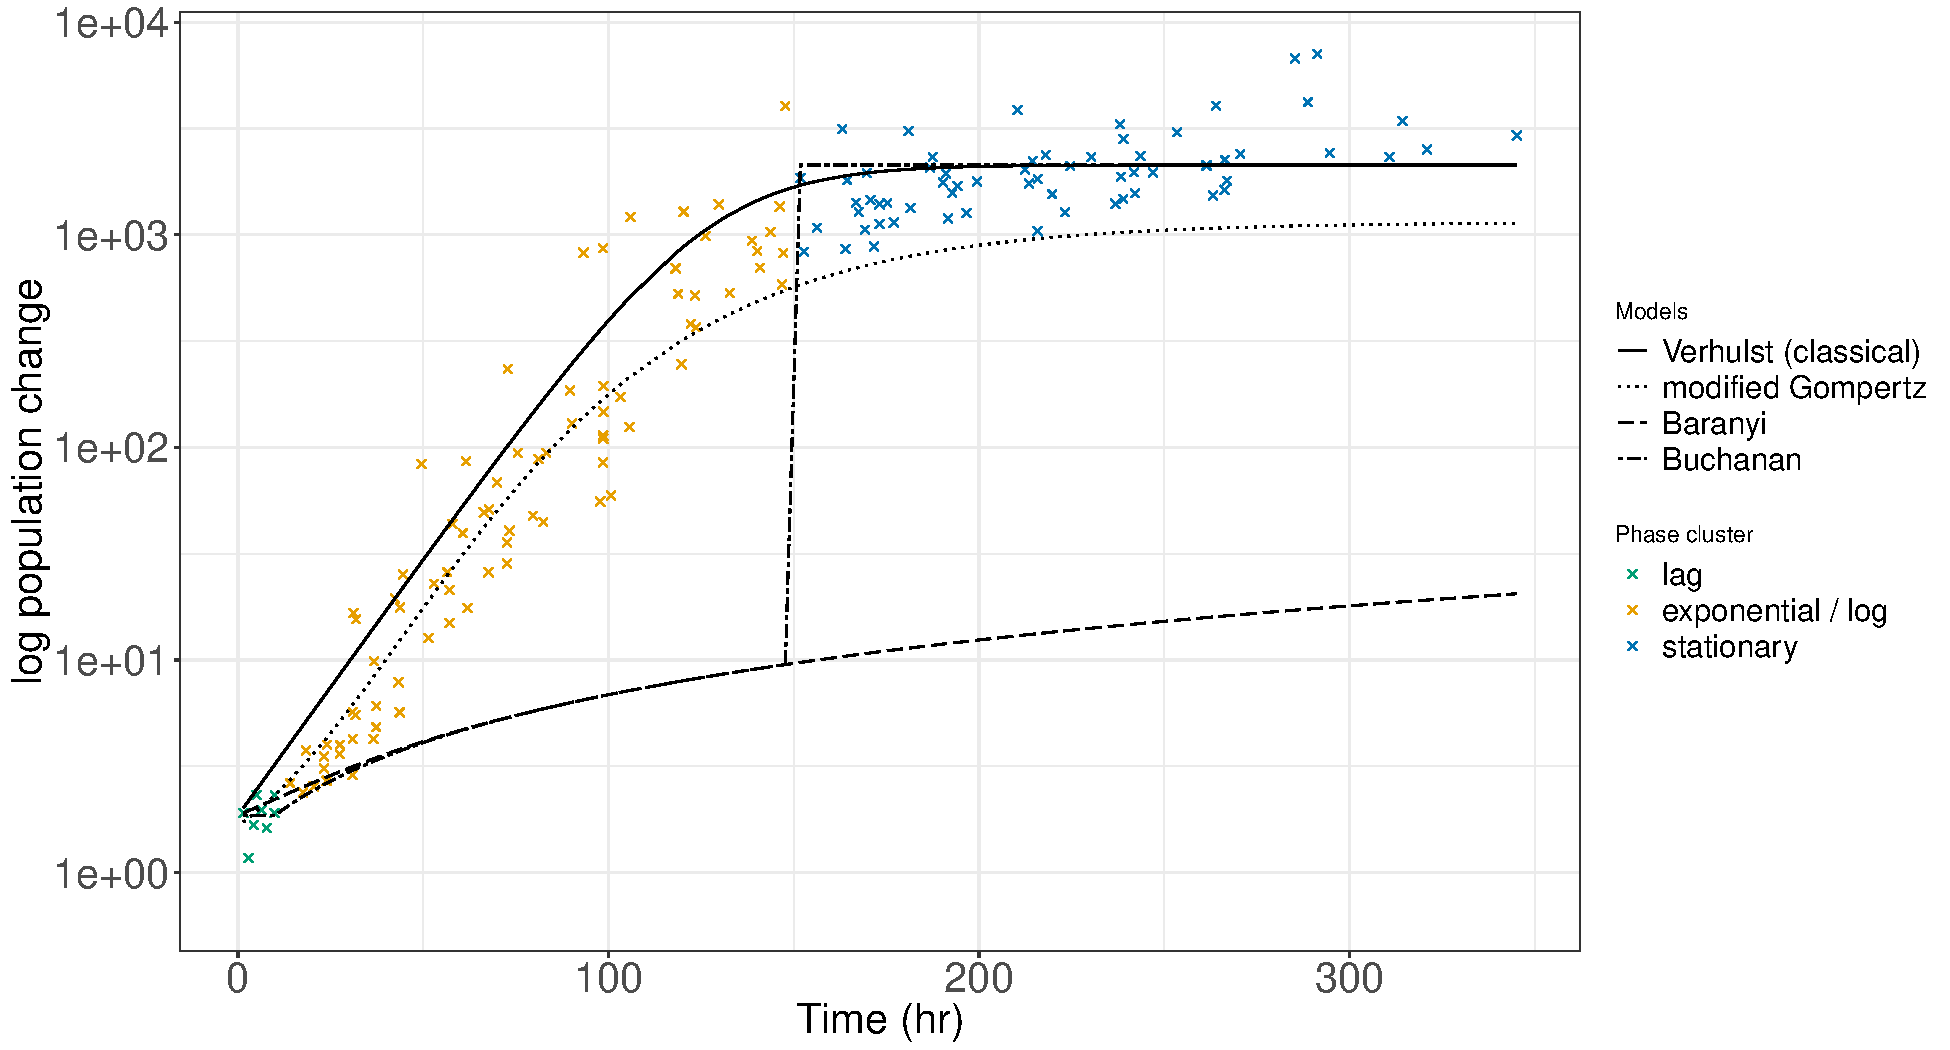
\includegraphics[width=\linewidth]{Log_data.pdf}\label{semi-log}
		\caption{Semi-log graph showing four different models fitting on data of ``Population Change" against ``Experiment time" with points clustered into three main phases of sigmoid growth curve.}
	\end{figure}
	\section*{Discussion}
	%% AIC vs BIC <https://www.methodology.psu.edu/resources/AIC-vs-BIC/>
	%% AIC <https://en.wikipedia.org/wiki/Akaike_information_criterion#Comparison_with_BIC>
	%% BIC <https://en.wikipedia.org/wiki/Bayesian_information_criterion>
	Model fitness to real data and simplistic mathematics were favoured by both AIC\autocite{johnson2004model,akaike1998information,burnhamdr} and BIC\autocite{johnson2004model,turchin2003complex}.  Apart from that, BIC also takes account of sample size effect\autocite{johnson2004model,turchin2003complex}.\\
	comparisons in different fields\autocite{kuha2004aic,aho2014model,yang2005can,penny2012comparing,vrieze2012model,wang2006comparison,acquah2010comparison}
	
	\section*{Conclusion}
	Upon model comparisons through AIC\autocite{akaike1998information,burnhamdr} and BIC\autocite{schwarz1978estimating} model selection methods, XXX is the most suitable model for describing the selected dataset.
	\section*{Code and Data Availability}
	All \href{https://github.com/ph-u/CMEECourseWork_pmH/tree/master/MiniProject/code}{scripts} and \href{https://github.com/ph-u/CMEECourseWork_pmH/tree/master/MiniProject/data}{data} used for this report were publicity available at GitHub.
	\nocite{*}\printbibliography
\end{document}